\section{Experiments}
\label{sec:experiments}

We organize results around three questions:
(1)~which method best detects stagnation across deployment scenarios? (\S\ref{sec:main_results}--\S\ref{sec:robustness});
(2)~what drives label quality and cross-coding-agent transfer bottlenecks? (\S\ref{sec:lf_temporal}--\S\ref{sec:cmd_rep_ablation});
(3)~can temporal structure in LFs improve labels? (\S\ref{sec:temporal_label_models}).
Silver-label metrics (Tables~\ref{tab:main_results}--\ref{tab:cmd_rep_ablation}) reflect LF-agreement scores; the gold set (\S\ref{sec:gold_set}) provides non-circular stagnation detection accuracy.

\paragraph{Circular evaluation caveat.}
Structural features overlap with the signals LFs use to produce silver labels; hence in-domain structural F1 (0.995) reflects LF reverse-engineering, not ground-truth accuracy.
Cross-agent evaluation on OpenHands (0.967) and the gold set (\S\ref{sec:gold_set}) provide non-circular evidence (\S\ref{sec:circular}).

%-------------------------------------------------------------------
\subsection{Experimental Setup}
\label{sec:setup}

\paragraph{Datasets.}
Sliding windows of $k{=}5$ consecutive actions are extracted from SWE-Agent (54,809 windows, 28.5\% stagnation) \citep{jimenez2024swebench,yang2024sweagent} and OpenHands (150,652 windows, 20.9\% stagnation) \citep{wang2025openhands} trajectories on SWE-bench.
Silver labels are produced by majority vote; confidence equals the count of agreeing LFs (1--3).
Splits are at the trajectory level (70/15/15\%); evaluation uses conf${\geq}$2: $N{=}1{,}824$ (SWE-Agent) and $N{=}43{,}376$ (OH).

\paragraph{Detection methods.}
(1)~\textbf{Structural features}: 30 hand-crafted features (repetition rates, file operation counts, edit distances, output entropy) fed to Logistic Regression (LR), Random Forest (RF), and Gradient Boosting (GB).
(2)~\textbf{ProgressProbe}: Qwen3-Embedding-0.6B \citep{zhang2025qwen3embedding} embeddings (1024-dim) processed by a 2-layer GRU \citep{cho2014gru} with attention \citep{bahdanau2015attention} (hidden$=$256, dropout$=$0.1), early-stopped at epoch~3 with patience~5.
(3)~\textbf{Mean-pool + LR}: Mean-pooled Qwen3 embeddings with logistic regression.
(4)~\textbf{LLM-as-Judge}: Claude Sonnet 4.6 zero-shot window-level classification (\$11.66 API cost for the SWE test set).
(5)~\textbf{Cosine similarity}: Cosine distance between consecutive window embeddings with a validation-tuned threshold.
(6)~\textbf{N-gram cycle detector}: Flags stagnation when an exact n-gram ($n \in \{2,3\}$) of commands recurs within a window---a simple repetition baseline absent from our initial comparison.

\paragraph{Metrics.}
Macro-F1 is the primary metric. We also report per-class F1 for stagnation (F1\textsubscript{stag}) and progress (F1\textsubscript{prog}).

%-------------------------------------------------------------------
\subsection{Main Results}
\label{sec:main_results}

Table~\ref{tab:main_results} presents in-domain results on the SWE-Agent conf${\geq}$2 test set and cross-coding-agent transfer to OpenHands.

\begin{table*}[t]
\centering
\small
\begin{tabular}{l ccc cc}
\toprule
& \multicolumn{3}{c}{\textbf{SWE-Agent In-Domain} (conf${\geq}$2)} & \multicolumn{2}{c}{\textbf{OpenHands Transfer}} \\
\cmidrule(lr){2-4} \cmidrule(lr){5-6}
\textbf{Method} & Macro-F1 & F1\textsubscript{stag} & F1\textsubscript{prog} & All & Conf${\geq}$2 \\
\midrule
Structural RF$^\dagger$       & \textbf{0.9951} & 0.9928 & 0.9974 & 0.9123 & \textbf{0.9959} \\
Structural GB$^\dagger$       & \textbf{0.9951} & 0.9928 & 0.9974 & \textbf{0.9674} & \underline{0.9918} \\
Structural LR$^\dagger$       & 0.9874 & 0.9815 & 0.9933 & 0.7801 & 0.9671 \\
ProgressProbe (GRU)           & \underline{0.9055} & 0.8593 & 0.9518 & 0.530$^a$ & 0.598$^a$ \\
\quad + full OH fine-tune      & ---    & ---    & ---    & 0.976$^b$ & 0.976$^b$ \\
Mean-pool + LR                & 0.8435 & 0.7620 & 0.9250 & ---    & --- \\
LLM-as-Judge                  & 0.6625 & 0.6055 & 0.7195 & ---    & --- \\
Cosine Similarity             & 0.5606 & ---    & ---    & 0.447  & 0.393 \\
\bottomrule
\end{tabular}
\caption{Stagnation detection results (SWE-Agent in-domain, $N{=}1{,}824$; OpenHands zero-shot transfer). $^\dagger$Structural metrics reflect LF-reconstructibility, not ground-truth accuracy (\S\ref{sec:circular}). $^a$Probe All: full OH embeddings ($N{=}143{,}057$); Conf${\geq}$2: 15\% test split ($N{=}6{,}122$). Structural models on all OH windows ($N{=}150{,}652$) and conf${\geq}$2 ($N{=}43{,}376$). $^b$Paired bootstrap ($N{=}6{,}122$): GB leads fine-tuned probe by 1.65\,pp (CI [1.11, 2.23], $p{<}0.001$) on conf${\geq}$2; probe advantage on all windows reflects better conf${=}1$ performance. \textbf{Bold} = best, \underline{underline} = second.}
\label{tab:main_results}
\end{table*}

In-domain, structural RF achieves 0.995 macro-F1, exceeding the GRU probe by 8.96\,pp (paired bootstrap: 95\% CI [7.44, 10.57]\,pp, $p{<}0.001$).
However, the structural--probe gap is inflated by circular evaluation: structural features reconstruct the LFs that generated the labels.
The more informative comparison is among non-circular methods: the GRU probe outperforms mean-pool~+~LR by 6.2\,pp, confirming that temporal modeling within windows adds value beyond static embedding aggregation.
The zero-shot LLM judge (0.663) underperforms all learned methods despite higher cost (\$11.66 per test set).
Extended evaluation (Appendix~\ref{sec:llm_extended}) yields a best LLM macro-F1 of 0.799 on silver (five-shot-CoT); on gold, the ranking reverses: LLM 0.910 surpasses structural GB 0.839 (\S\ref{sec:gold_set}), illustrating silver-label circularity.
CoT and few-shot yield comparable gains ($+$8.7 vs.\ $+$8.9\,pp); combining them adds $+$4.8\,pp.

%-------------------------------------------------------------------
\subsection{Cross-Agent Transfer}
\label{sec:cross_agent}

Table~\ref{tab:main_results} (right columns) shows models trained on SWE-Agent and evaluated on OpenHands without any OH training data.
Structural GB transfers best, achieving 0.967 macro-F1 on all OH windows.
RF drops to 0.912 on all-confidence OH data despite matching GB in-domain, suggesting GB's boosted ensemble is more robust to distributional shift.
Both structural models exceed 0.99 macro-F1 on conf${\geq}$2 OH windows (GB 0.992, RF 0.996), where label noise is lower.
Transfer is symmetric: OH$\to$SWE achieves 0.995 for both GB and RF on conf${\geq}$2, comparable to SWE$\to$OH (0.992/0.996), confirming agent-agnostic structural patterns (Appendix Table~\ref{tab:reverse_transfer}).
The LLM judge degrades further on OH (0.491 zero-shot; $N{=}500$), 47.6\,pp below structural GB---few-shot-CoT (0.470) underperforms zero-shot, as SWE-Agent examples induce negative transfer.

On the same OH conf${\geq}$2 test split ($N{=}6{,}122$), the probe's zero-shot transfer (0.598) lags structural GB (0.993) by 39.4\,pp (95\% CI [37.9, 41.0]), but full OH fine-tuning closes this gap: the fine-tuned probe reaches 0.976, surpassing GB (0.967) on all windows (\S\ref{sec:cmd_rep_ablation}).
The practical implication is a deployment trade-off: structural features when no labeled data is available; probe fine-tuning when annotation budget permits.
This crossover is scope-dependent: on conf${\geq}$2, GB retains its advantage (0.992 vs.\ 0.976; $p{<}0.001$), suggesting the probe's all-windows edge reflects tolerance of noisy conf${=}1$ labels rather than superior detection.

\paragraph{Multi-seed stability.}
Structural RF: $0.995{\pm}0.000$ in-domain (3 seeds); GB cross-coding-agent: $0.968{\pm}0.002$.
The probe shows higher variance ($0.919{\pm}0.011$) but all seeds exceed 0.90.

%-------------------------------------------------------------------
\subsection{Robustness Analysis}
\label{sec:robustness}

In-domain performance is encoder-agnostic (0.93--0.94 across three encoders; Appendix Table~\ref{tab:encoder_ablation}), and a Transformer encoder is equivalent to GRU ($+$0.18\,pp, $p{=}0.82$).
Cross-agent transfer varies with encoder choice (0.60--0.73, 13.5\,pp spread), but even the best probe (E5-large, 0.733) remains 25.9\,pp below structural GB (0.992), confirming the structural advantage is robust across encoders (Appendix Table~\ref{tab:encoder_cross}).
Window size $k{=}5$ is optimal; $k{=}3$ drops 5.9\,pp, $k{=}7$ drops 1.8\,pp (Appendix Table~\ref{tab:window_ablation}).
Structural classifiers are extremely data-efficient: RF achieves 0.991 and GB 0.987 at just 10\% training data, fully saturating by 50\%---a 20$\times$ advantage over the probe (Figure~\ref{fig:data_scaling}).

\begin{figure}[t]
\centering
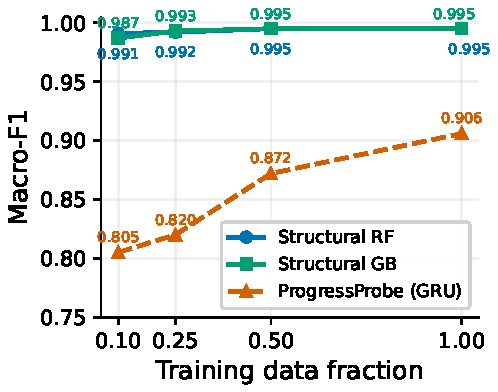
\includegraphics[width=0.9\columnwidth]{../../figures/paper/fig_data_scaling.pdf}
\caption{Macro-F1 vs.\ training data fraction. Structural classifiers saturate by 50\%; the probe has not plateaued at 100\%.}
\label{fig:data_scaling}
\end{figure}

%-------------------------------------------------------------------
\subsection{Labeling Function Temporal Dynamics}
\label{sec:lf_temporal}

The three LFs occupy distinct temporal niches (Table~\ref{tab:lf_temporal}, Figure~\ref{fig:lf_temporal} in Appendix~\ref{sec:app_lf_temporal}): cmd\_rep leads by 1.87 steps, file\_diff is near-concurrent ($-1.20$), and outcome\_bp lags by 6.70 steps (all pairwise $p{<}10^{-26}$).
On OpenHands, cmd\_rep reverses to lagging ($+3.32$ steps), firing on only 5.4\% of windows with 97.9\% precision---a fundamentally different temporal role than on SWE-Agent.

%-------------------------------------------------------------------
\subsection{Label Quality and cmd\_rep Coverage}
\label{sec:cmd_rep_ablation}

A label quality audit revealed a version mismatch in OH embedding vectors; after correction, the OH stagnation rate shifted from 6.56\% to 21.4\%, and 5\% fine-tuning F1 improved from 0.570 to 0.850---demonstrating that label quality, not model capacity, was the transfer bottleneck (full curve in Appendix Table~\ref{tab:cross_agent_cmdrep}).

\begin{table}[t]
\centering
\small
\begin{tabular}{lccc}
\toprule
\textbf{LF Config} & \textbf{Macro-F1} & \textbf{F1\textsubscript{stag}} & \textbf{F1\textsubscript{prog}} \\
\midrule
3-LF (w/ cmd\_rep) & \textbf{0.9763} & 0.9600 & 0.9930 \\
2-LF (no cmd\_rep) & 0.6822 & 0.4810 & 0.8840 \\
\midrule
$\Delta$ & $-29.4$\,pp & $-47.9$\,pp & $-10.9$\,pp \\
\bottomrule
\end{tabular}
\caption{Prevalence-matched ablation on the same OH test set ($N{=}6{,}122$, stag rate 19.3\%). Removing cmd\_rep drops macro-F1 by 29.4\,pp (McNemar $\chi^2{=}1551$, $p{\approx}0$).}
\label{tab:cmd_rep_ablation}
\end{table}

Removing cmd\_rep drops macro-F1 by 29.4\,pp (Table~\ref{tab:cmd_rep_ablation}; McNemar $p{\approx}0$) due to data volume collapse: cmd\_rep expands training data ${\sim}$10$\times$ (4K$\to$43K windows) while agreeing 100\% with 2-LF labels on overlapping windows---purely a coverage contribution (Appendix~\ref{sec:app_label_quality}).

%-------------------------------------------------------------------
\subsection{Temporal Label Models}
\label{sec:temporal_label_models}

Five label models---three temporal (TWV, HMM, Lag-HMM) and two generative (FlyingSquid, Snorkel MeTaL)---all fail to improve over majority vote (Table~\ref{tab:temporal_models} in Appendix~\ref{sec:app_tlm_results}); the best (TWV, $+$0.6\,pp self-evaluated) degrades downstream probe F1 by 2.57\,pp.
The bottleneck is LF quantity: three binary LFs produce at most $2^3{=}8$ voting patterns with insufficient inter-LF conflict to exploit.
A 6-LF expansion confirms this: HMM recovers $+$6.5\,pp but remains below 3-LF MV in absolute terms (Appendix~\ref{sec:app_6lf}).

%-------------------------------------------------------------------
\subsection{Gold Set Validation}
\label{sec:gold_set}
Three CS graduate students annotate a stratified gold set ($N{=}505$, ${\geq}$2 annotators agree, stagnation prevalence 26.3\% vs.\ silver 24.6\%; silver--gold agreement 93.8\%, $\kappa{=}0.865$; protocol in Appendix~\ref{sec:app_gold_set}).
GB achieves 0.839 gold macro-F1 vs.\ 0.798 for MV ($+$4.2\,pp, bootstrap $p{<}0.001$, 95\% CI [0.758, 0.837]); probe models use the SWE-only subset ($N{\approx}335$, Table~\ref{tab:gold_batch1}).

\paragraph{LLM gold evaluation.}
The best LLM (few-shot-CoT) achieves 0.910 gold macro-F1, surpassing GB (0.839) by 7.1\,pp---reversing the silver ranking---but LLM judges collapse on cross-agent transfer (best: 0.491 vs.\ 0.967, $-$47.6\,pp; \S\ref{sec:cross_agent}).

\paragraph{Cycle detector comparison.}
N-gram cycle detectors match structural GB on in-domain gold (${\sim}$0.84) but collapse cross-agent ($-$43.7\,pp; Appendix Table~\ref{tab:cycle_detector}).